% 컴파일: latexmk -xelatex main.tex  (XeLaTeX + kotex 필요)
\documentclass[11pt,a4paper]{article}

\usepackage{kotex}
\setmainhangulfont{AppleMyungjo}[BoldFont={Apple SD Gothic Neo Bold}]
\setsanshangulfont{Apple SD Gothic Neo}

\usepackage[margin=25mm]{geometry}
\usepackage{graphicx}
\usepackage{booktabs}
\usepackage{amsmath}
\usepackage{siunitx}
\usepackage[hidelinks]{hyperref}
\usepackage{caption}
\captionsetup{font=small, labelfont=bf}

\graphicspath{{figures/}}

\title{다층 신경망을 이용한 SDSS 천체 분류:\\데이터 탐색과 베이스라인 설계}
\author{이인수}
\date{2026년 7월 7일}

\begin{document}
\maketitle

\begin{abstract}
Sloan Digital Sky Survey(SDSS) 관측 데이터 10만 건을 이용해 천체를 은하(GALAXY),
별(STAR), 퀘이사(QSO)의 세 클래스로 분류하는 다층 신경망 모델을 구축하기에 앞서,
데이터셋의 탐색적 분석과 전처리 방침 수립, 그리고 은닉층 깊이 선정 실험을 수행하였다.
결측치는 SDSS 오류 센티널 값($-9999$)을 갖는 1개 행뿐이어서 제거하였고, IQR 기준
이상치는 클래스별 교차 분석 결과 적색편이(redshift) 이상치의 99.6\%가 QSO에
집중되어 있어 제거 대상이 아닌 판별 신호로 판단하였다. 은닉층 0--3개 구성을 비교한
실험에서 은닉층 2개(64, 32) 구조가 검증 macro-F1 $0.9681 \pm 0.0016$으로 가장
우수하였으며, 깊이를 더 늘려도 성능 향상이 없어 이를 베이스라인 구조로 채택하였다.
채택 구조를 PyTorch로 재구현한 뒤 클래스 가중치와 색지수 파생 특성의 효과를 절제
실험으로 검증한 결과, 색지수 4개를 추가한 구성이 가장 우수하여 이를 최종 구성으로
확정하였고 시험 세트에서 macro-F1 $0.9700 \pm 0.0002$를 얻었다. 마지막으로 무작위
시드로 학습한 동일 모델 10개의 과반수 투표 앙상블은 시험 macro-F1 0.9703으로 개별
모델의 시드 간 변동을 제거하였다.
\end{abstract}

\section{서론}

본 연구의 목표는 SDSS 측광·분광 관측치로부터 천체의 종류를 자동 분류하는 다층
신경망(multilayer neural network) 모델을 구축하는 것이다. 본 보고서는 (1) 데이터셋
탐색, (2) 결측치·이상치 분석과 전처리 방침 수립, (3) 클래스별 특성 분포 비교,
(4) 은닉층 깊이 선정 실험, (5) PyTorch 전환과 클래스 가중치·색지수 파생 특성의
절제(ablation) 실험 및 시험 세트 평가, (6) 과반수 투표 앙상블 실험의 과정과 결과를
정리한다.

\section{데이터셋}

데이터셋(\texttt{star\_classification.csv})은 SDSS 관측 천체 100{,}000건으로,
17개 특성 컬럼과 타깃 \texttt{class}로 구성된다. 클래스 분포는 GALAXY 59{,}445건
(59.4\%), STAR 21{,}594건 (21.6\%), QSO 18{,}961건 (19.0\%)으로 불균형하다.
특성은 표~\ref{tab:features}와 같이 구분된다. 식별자·메타데이터 컬럼은 물리적
의미가 없으므로 모델 입력에서 제외하고, 수치형 특성 8개를 분석 대상으로 삼았다.

\begin{table}[htbp]
\centering
\caption{특성 구분과 타입}
\label{tab:features}
\small
\begin{tabular}{lll}
\toprule
구분 & 컬럼 & 타입 \\
\midrule
측광 (magnitude) & \texttt{u, g, r, i, z} & float64 \\
분광 & \texttt{redshift} & float64 \\
위치 & \texttt{alpha}(적경), \texttt{delta}(적위) & float64 \\
식별자·메타데이터 & \texttt{obj\_ID, spec\_obj\_ID} & float64 \\
식별자·메타데이터 & \texttt{run\_ID, rerun\_ID, cam\_col, field\_ID,} & int64 \\
 & \texttt{plate, MJD, fiber\_ID} & \\
타깃 & \texttt{class} & GALAXY / STAR / QSO \\
\bottomrule
\end{tabular}
\end{table}

\section{데이터 품질 분석}

\subsection{결측치}

NaN 형태의 결측치는 전 컬럼에서 0개였다. 다만 1개 행(index 79543)의
\texttt{u, g, z}에 SDSS 오류 센티널 값 $-9999$가 존재하여 사실상의 결측으로
판단하였다. 전체의 0.001\%에 불과하므로 대치 대신 행 삭제를 택했다.

\subsection{수치형 특성 분포}

그림~\ref{fig:dist}은 수치형 특성 8개의 분포이다(센티널 제외). 측광 특성
\texttt{g, r, i, z}는 쌍봉(bimodal) 형태를 보이는데, 이는 4절에서 확인하듯
클래스 혼합이 원인이다. \texttt{redshift}는 0 부근의 큰 스파이크(별)와 최대
7.01까지 이어지는 긴 오른쪽 꼬리(QSO)를 갖는 심한 우측 왜도 분포로, 스케일링
전 변환이 필요하다. 위치 특성 \texttt{alpha, delta}는 서베이 커버리지를 반영할
뿐 클래스와 물리적 연관이 없어 특성에서 제외하였다.

\begin{figure}[htbp]
\centering
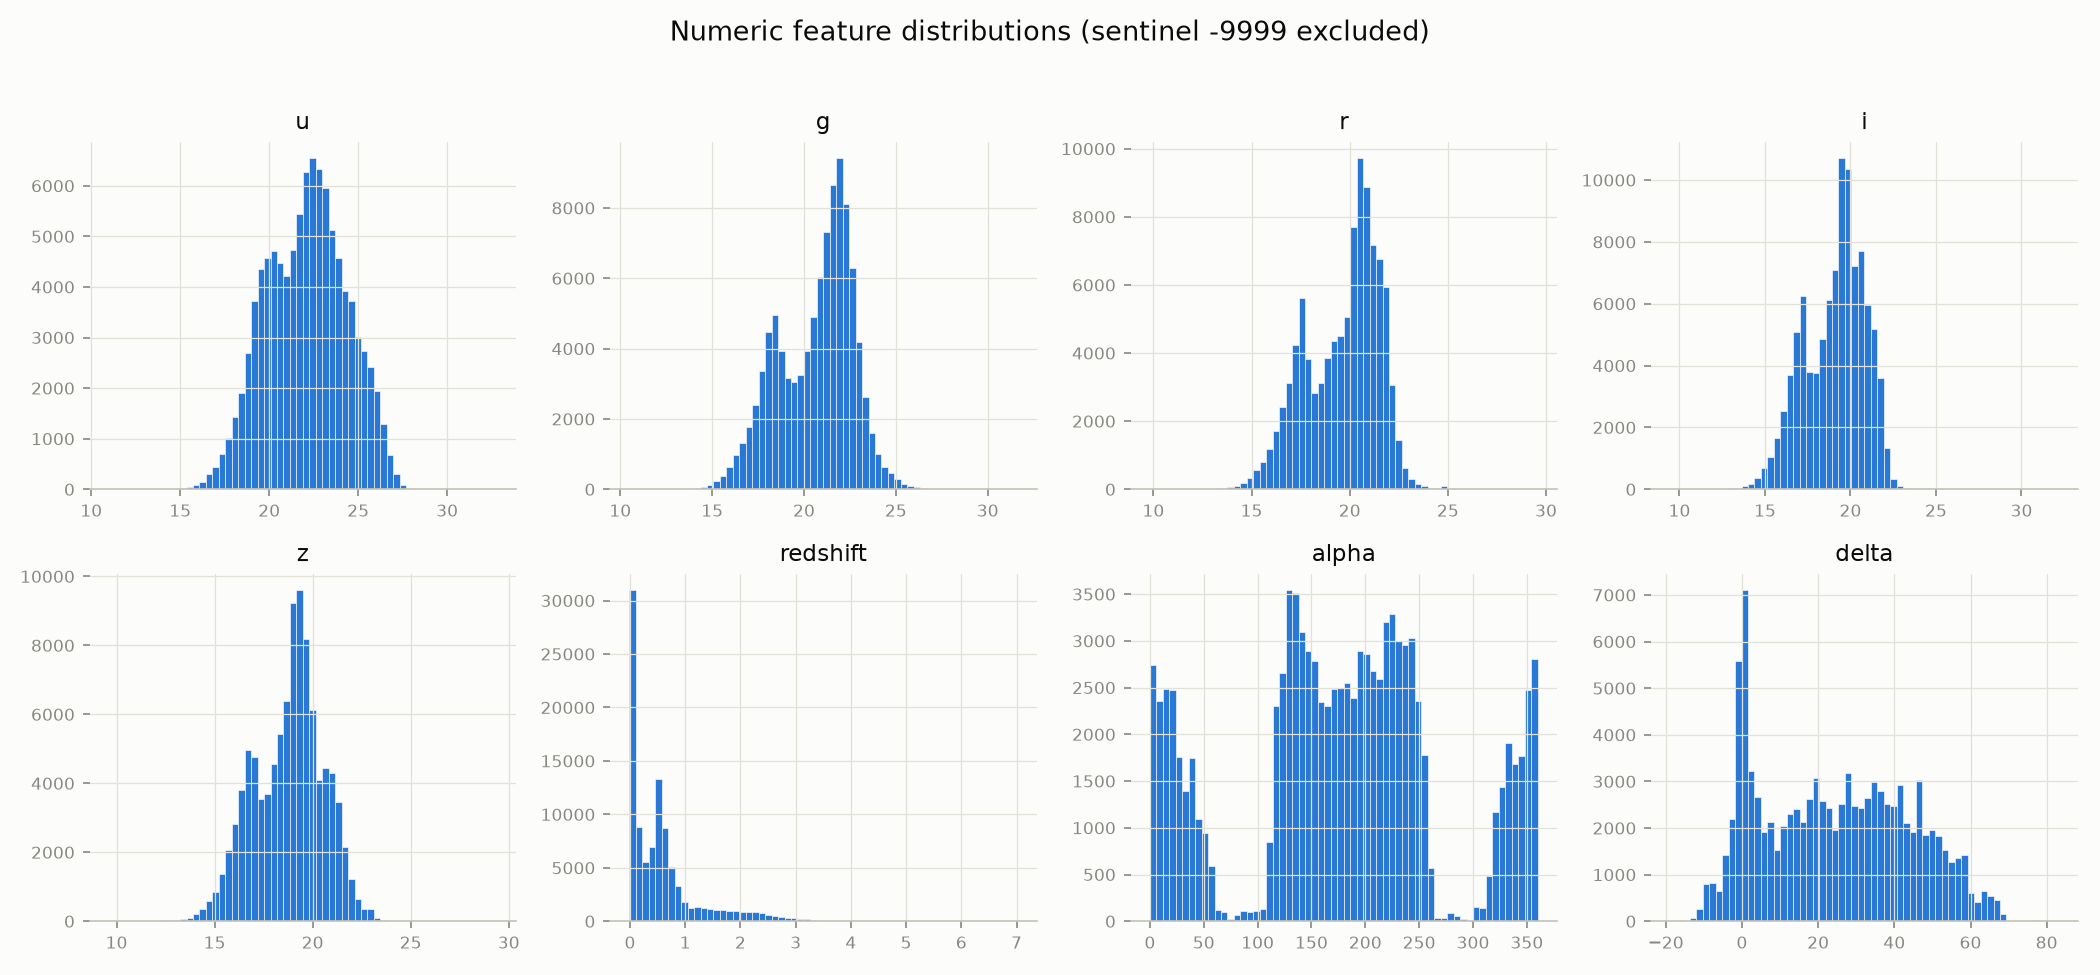
\includegraphics[width=\textwidth]{numeric_distributions.png}
\caption{수치형 특성 8개의 분포 (센티널 $-9999$ 제외).}
\label{fig:dist}
\end{figure}

\subsection{이상치 탐지와 클래스별 교차 분석}

그림~\ref{fig:box}의 boxplot과 $1.5\times$IQR 기준으로 이상치를 탐지한 결과,
측광 특성의 이상치는 0.06--0.32\%로 소수였으나 \texttt{redshift}는 8{,}990건
(8.99\%)이 검출되었다. 이 ``이상치''가 노이즈인지 신호인지 판별하기 위해
클래스별 교차 분석을 수행하였다(표~\ref{tab:outlier-class}).

\begin{figure}[htbp]
\centering
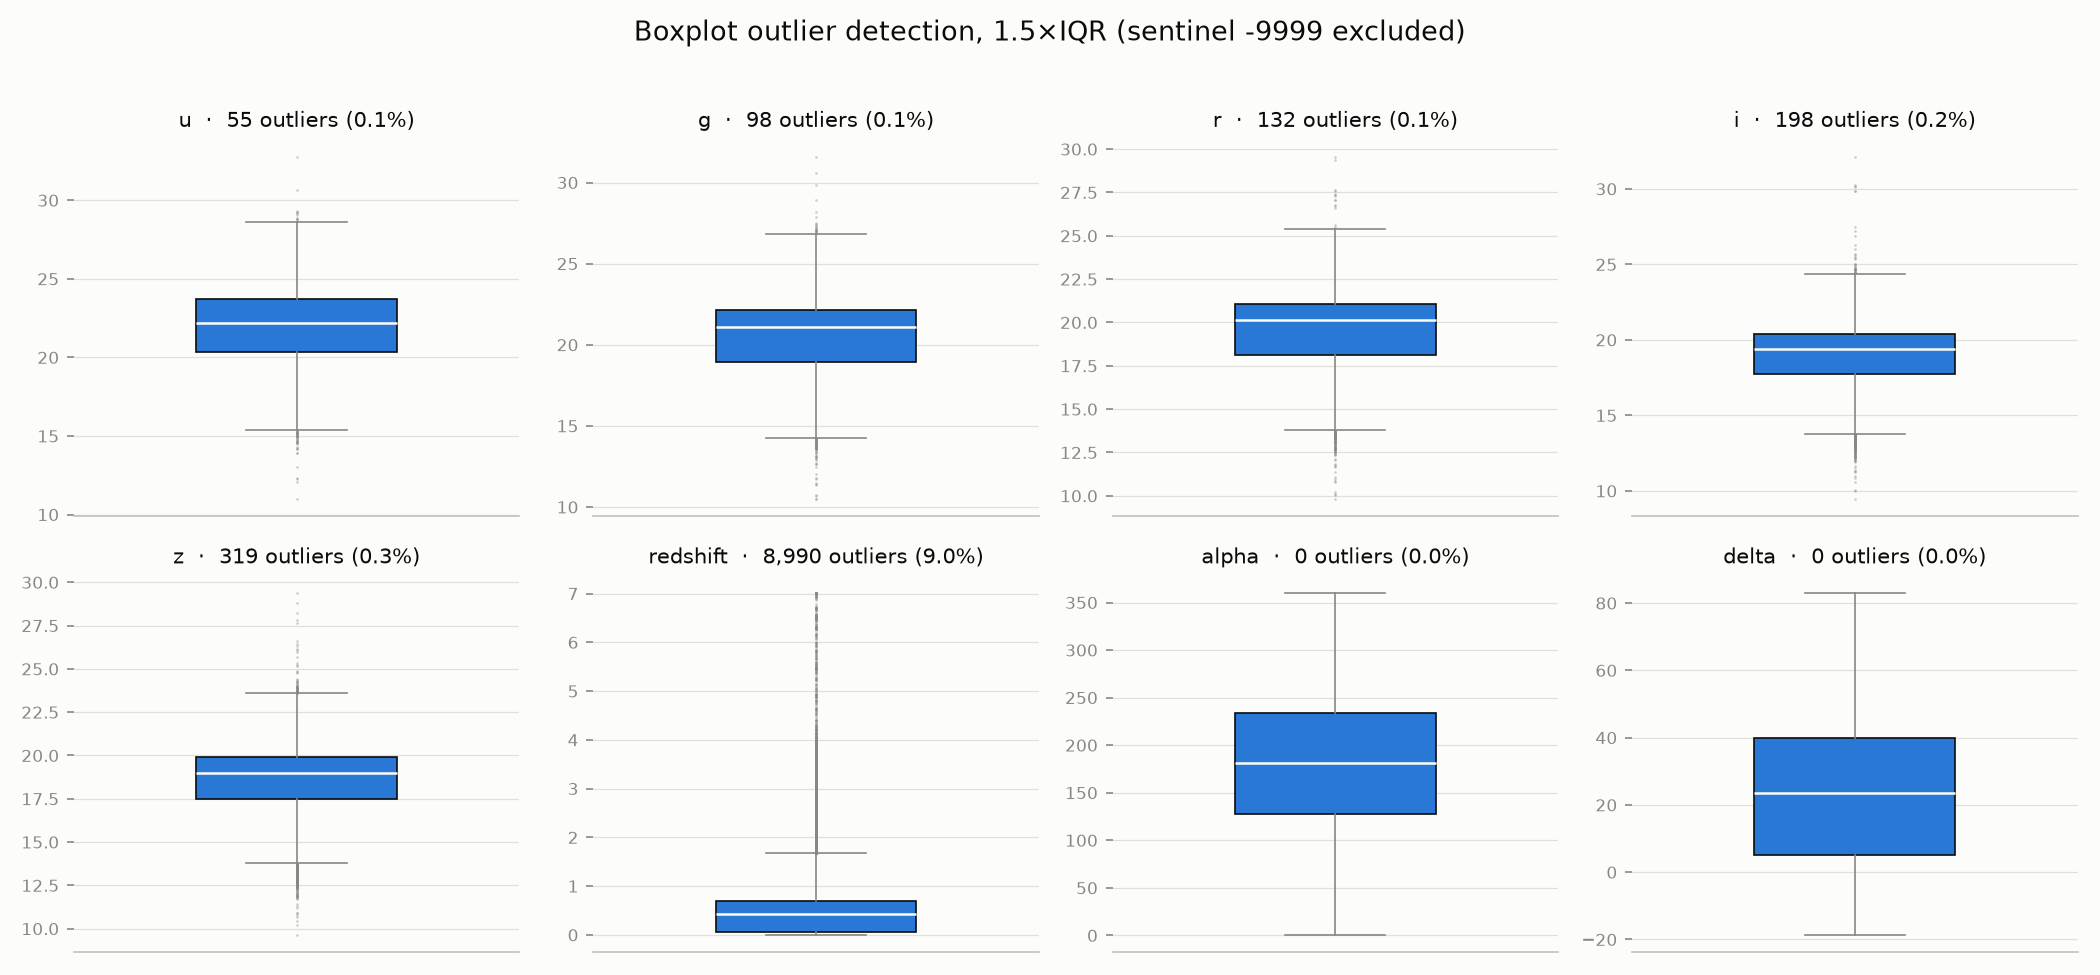
\includegraphics[width=\textwidth]{outliers_boxplot.png}
\caption{특성별 boxplot 기반 이상치 탐지 ($1.5\times$IQR, 센티널 제외).}
\label{fig:box}
\end{figure}

\begin{table}[htbp]
\centering
\caption{IQR 이상치의 클래스 구성. 기저 비율은 GALAXY 59.4\% / STAR 21.6\% / QSO 19.0\%.}
\label{tab:outlier-class}
\small
\begin{tabular}{lrrrr}
\toprule
특성 & 이상치 수 & GALAXY & STAR & QSO \\
\midrule
\texttt{u} & 55 & 36.4\% & 58.2\% & 5.5\% \\
\texttt{g} & 98 & 68.4\% & 26.5\% & 5.1\% \\
\texttt{r} & 132 & 69.7\% & 27.3\% & 3.0\% \\
\texttt{i} & 198 & 76.3\% & 16.7\% & 7.1\% \\
\texttt{z} & 319 & 77.4\% & 17.2\% & 5.3\% \\
\texttt{redshift} & 8{,}990 & 0.4\% & 0.0\% & \textbf{99.6\%} \\
\bottomrule
\end{tabular}
\end{table}

\texttt{redshift} 이상치 8{,}990건 중 99.6\%(8{,}956건)가 QSO였다. 즉 IQR
기준이 분포 왜도 때문에 고적색편이 QSO를 과탐지한 것으로, 이는 제거해야 할
노이즈가 아니라 클래스 판별의 핵심 신호이다. 그림~\ref{fig:rbc}에서 보듯 세
클래스의 redshift 분포는 뚜렷이 분리된다(STAR $\approx 0$, GALAXY 중앙값
$\sim$0.42, QSO 중앙값 $\sim$1.6). 측광 특성의 이상치 역시 기저 비율과 다른
클래스 편향을 보여 무작위 노이즈가 아니므로, 이상치는 일괄 제거하지 않기로
결정하였다.

\begin{figure}[htbp]
\centering
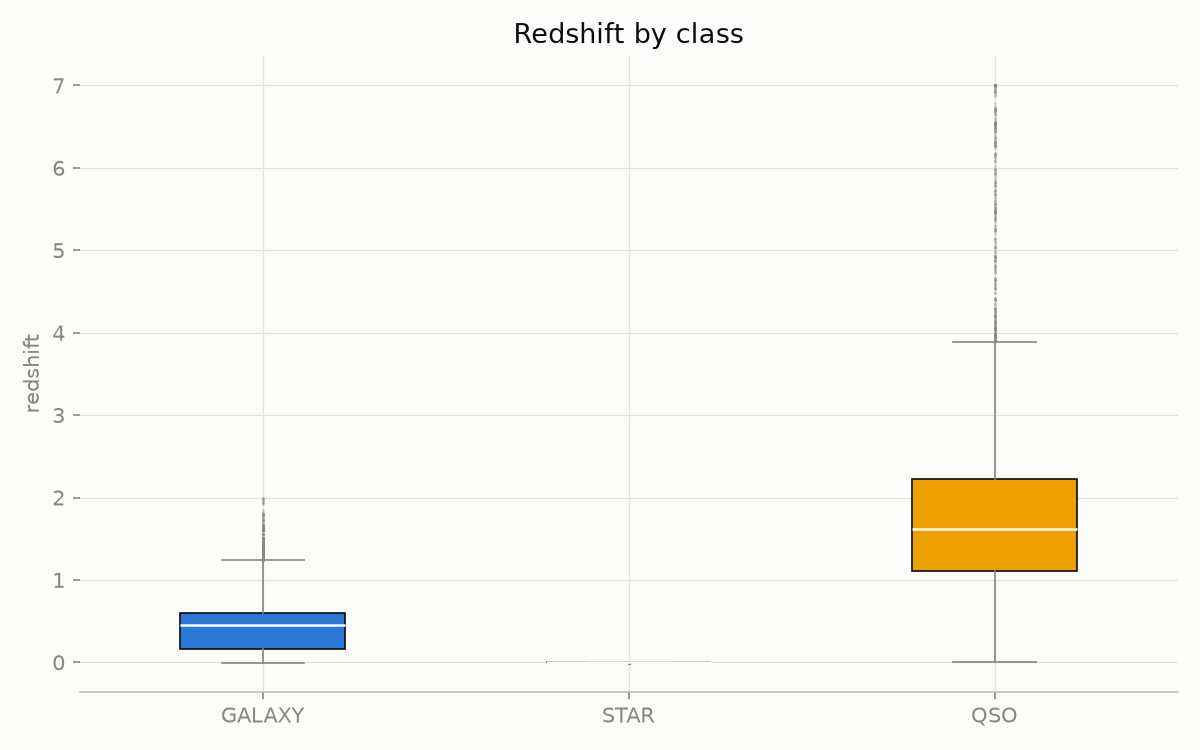
\includegraphics[width=0.75\textwidth]{redshift_by_class.png}
\caption{클래스별 redshift 분포. 세 클래스가 redshift만으로도 크게 분리된다.}
\label{fig:rbc}
\end{figure}

\section{클래스별 측광·색지수 분포}

클래스 불균형의 영향을 배제하기 위해 밀도 정규화(density)된 히스토그램으로
클래스별 분포를 비교하였다. 그림~\ref{fig:mag}에서 전체 분포의 쌍봉이 클래스
혼합의 결과임이 확인되며, 클래스별 분포는 대체로 단봉이다. QSO는
\texttt{r, i, z}에서 체계적으로 어둡고(중앙값 20.4--20.8), STAR는 밝은 쪽에
분포한다.

\begin{figure}[htbp]
\centering
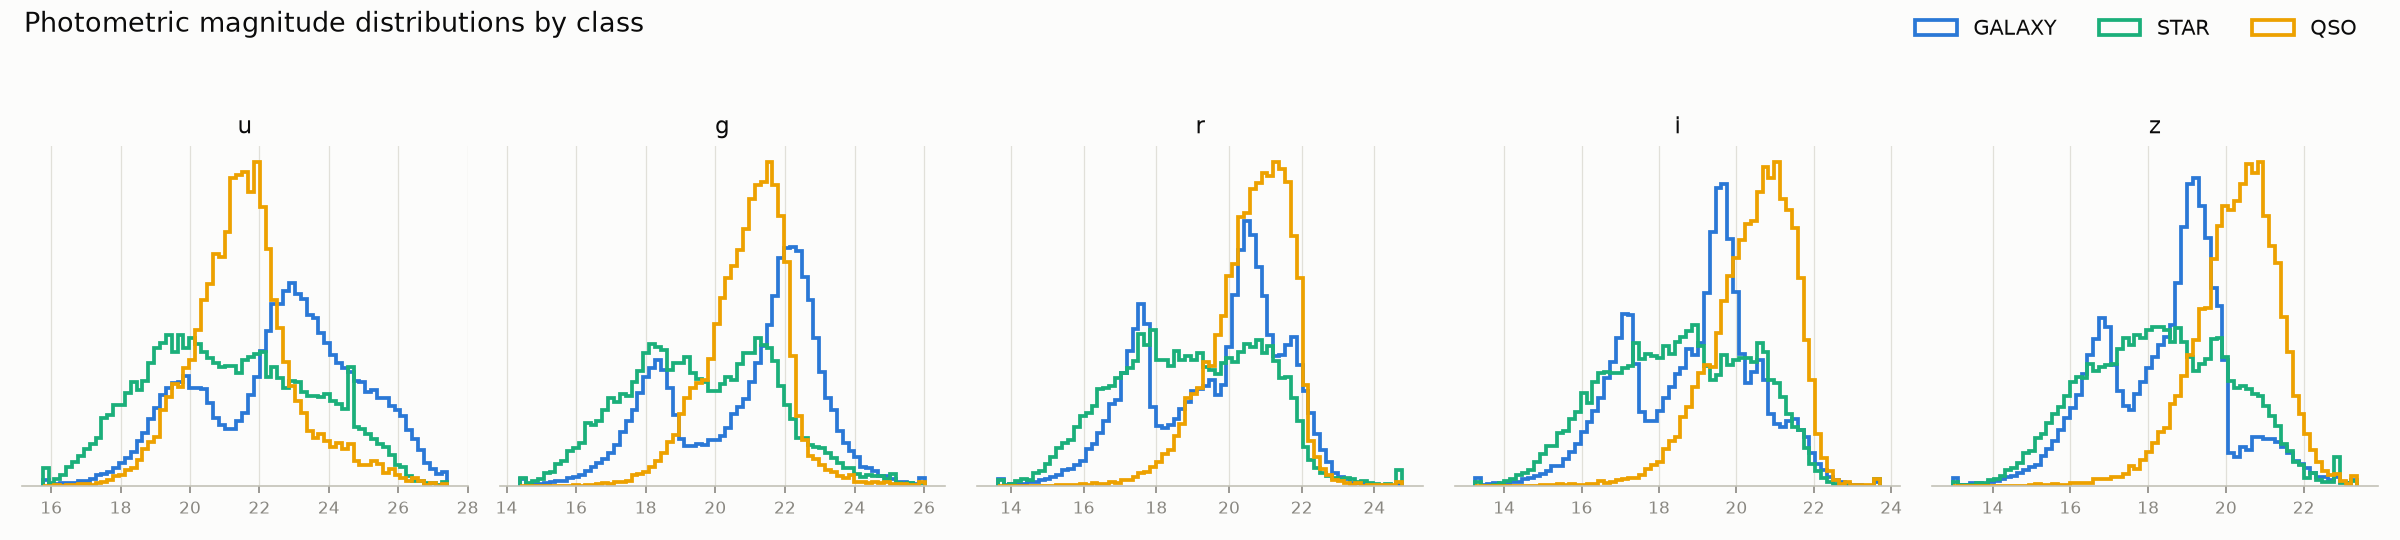
\includegraphics[width=\textwidth]{magnitudes_by_class.png}
\caption{클래스별 측광 특성 분포 (밀도 정규화).}
\label{fig:mag}
\end{figure}

인접 밴드 차로 정의한 색지수(color index) $u-g$, $g-r$, $r-i$, $i-z$는
클래스를 잘 분리한다(그림~\ref{fig:ci}, 표~\ref{tab:medians}). QSO는 가장
파랗고($u-g$ 중앙값 0.39), GALAXY는 가장 붉으며($u-g$ 1.64, $g-r$ 1.40),
STAR는 그 중간이다. GALAXY의 $g-r$ 쌍봉은 red sequence / blue cloud로 해석할
수 있다. 색지수는 redshift에 덜 의존하는 판별력을 제공할 수 있어 파생 특성
후보로 유망하다.

\begin{figure}[htbp]
\centering
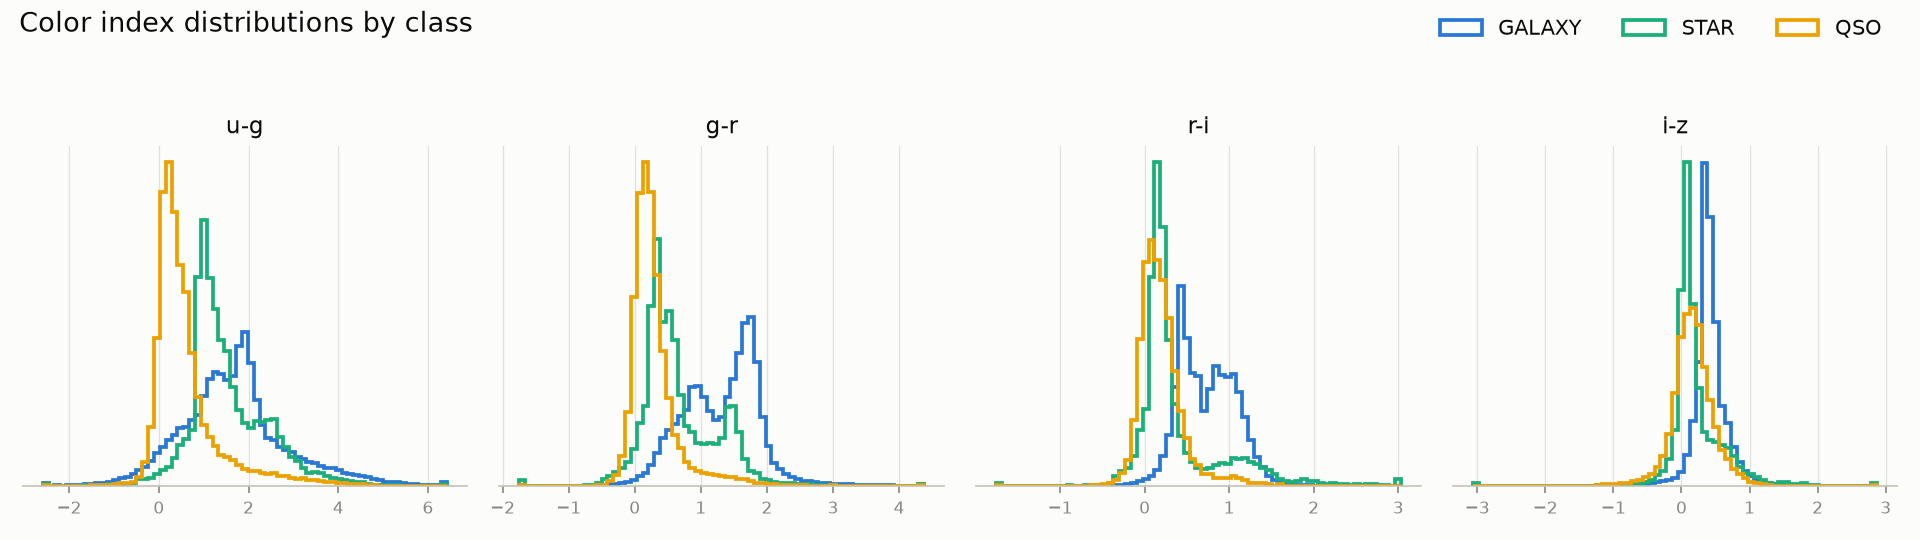
\includegraphics[width=\textwidth]{color_indices_by_class.png}
\caption{클래스별 색지수 분포 (밀도 정규화).}
\label{fig:ci}
\end{figure}

\begin{table}[htbp]
\centering
\caption{클래스별 측광 특성·색지수 중앙값}
\label{tab:medians}
\small
\begin{tabular}{lrrrrrrrrr}
\toprule
class & $u$ & $g$ & $r$ & $i$ & $z$ & $u-g$ & $g-r$ & $r-i$ & $i-z$ \\
\midrule
GALAXY & 22.84 & 21.58 & 20.11 & 19.22 & 18.77 & 1.640 & 1.404 & 0.720 & 0.391 \\
STAR   & 21.01 & 19.54 & 18.96 & 18.59 & 18.32 & 1.319 & 0.527 & 0.211 & 0.116 \\
QSO    & 21.50 & 21.06 & 20.77 & 20.58 & 20.37 & 0.393 & 0.214 & 0.152 & 0.157 \\
\bottomrule
\end{tabular}
\end{table}

\section{전처리 방침}

이상의 분석을 근거로 다음 네 가지 전처리 방침을 확정하였다
(\texttt{preprocess.py}로 구현).

\begin{enumerate}
  \item \textbf{결측치}: 센티널 행(index 79543) 삭제 $\rightarrow$ 99{,}999행.
  \item \textbf{이상치}: 제거하지 않음. redshift 이상치는 QSO 판별 신호이며,
        측광 이상치는 0.3\% 이하의 소수로 물리적으로 유효한 천체일 가능성이 높다.
  \item \textbf{특성 선택}: 식별자·메타데이터 컬럼과 \texttt{alpha, delta} 제외
        $\rightarrow$ \texttt{u, g, r, i, z, redshift} 6개.
  \item \textbf{스케일링}: \texttt{redshift}는 $\log(1+x)$ 변환(최솟값 $-0.01$이라
        안전) 후 표준화, 측광 5개는 꼬리의 영향이 적은 중앙값/IQR 기반
        RobustScaler. 스케일러는 학습 분할에만 적합(fit)하여 정보 누수를 방지한다.
\end{enumerate}

\section{은닉층 깊이 선정 실험}

입력이 6차원인 저차원 정형 데이터이므로 깊은 네트워크가 필요하지 않다는 가설을
실험으로 검증하였다. 데이터를 학습 64{,}000 / 검증 16{,}000 / 시험 20{,}000건으로
층화 분할하고(시험 세트는 최종 평가용으로 미사용), scikit-learn
\texttt{MLPClassifier}(ReLU, Adam, 배치 512, 조기 종료)로 은닉층 0--3개 구성을
비교하였다. 무작위성을 고려해 MLP는 서로 다른 시드 3개의 평균을 보고한다.

\begin{table}[htbp]
\centering
\caption{은닉층 깊이별 검증 성능 (시드 3개 평균 $\pm$ 표준편차)}
\label{tab:depth}
\small
\begin{tabular}{lccc}
\toprule
구성 & 검증 macro-F1 & 검증 정확도 & 학습 시간 \\
\midrule
로지스틱 회귀 (0층) & 0.9531 & 0.9594 & \SI{0.3}{s} \\
MLP 1층 (64) & $0.9660 \pm 0.0010$ & 0.9705 & \SI{2.9}{s} \\
\textbf{MLP 2층 (64, 32)} & $\mathbf{0.9681 \pm 0.0016}$ & \textbf{0.9723} & \SI{3.6}{s} \\
MLP 3층 (64, 32, 16) & $0.9675 \pm 0.0016$ & 0.9718 & \SI{2.9}{s} \\
\bottomrule
\end{tabular}
\end{table}

\begin{figure}[htbp]
\centering
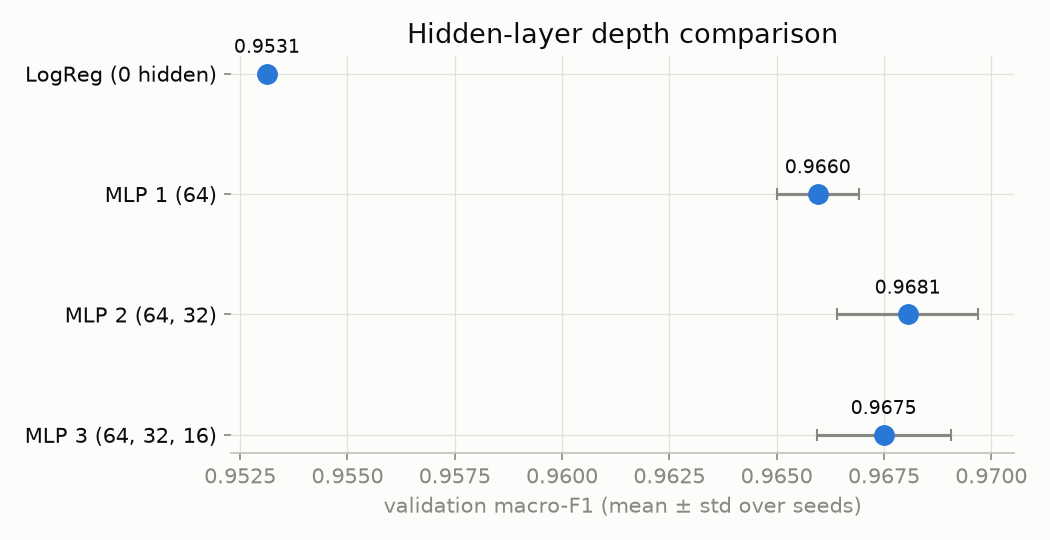
\includegraphics[width=0.8\textwidth]{depth_comparison.png}
\caption{은닉층 깊이별 검증 macro-F1 (시드 3개 평균 $\pm$ 표준편차).}
\label{fig:depth}
\end{figure}

표~\ref{tab:depth}와 그림~\ref{fig:depth}에서 비선형성의 효과는 뚜렷하다
(0층 $\rightarrow$ 1층에서 macro-F1 $+1.3$\%p). 반면 깊이의 효과는 미미하여
1층 $\rightarrow$ 2층은 $+0.2$\%p로 시드 표준편차와 비슷한 크기이고, 3층에서는
오히려 소폭 하락한다. 따라서 \textbf{은닉층 2개 (64, 32)}를 베이스라인 구조로
채택한다. 채택 구조의 클래스별 검증 F1은 GALAXY 0.977, STAR 0.988, QSO 0.940
(재현율 0.911)으로, QSO 재현율이 상대적 약점이다.

\section{모델 개선: 클래스 가중치와 색지수 파생 특성}

6절에서 확인한 QSO 재현율 약점을 개선하기 위해, 채택 구조를 PyTorch로
재구현하고(Adam $10^{-3}$, 배치 512, 검증 macro-F1 기준 조기 종료) 두 가지
개선안을 절제 실험으로 검증하였다: (a) 역빈도 클래스 가중치를 적용한
교차 엔트로피 손실, (b) 4절의 색지수 4개를 파생 특성으로 추가(입력 10차원).
분할은 6절과 동일하며, 각 구성은 시드 3개의 평균을 보고한다
(표~\ref{tab:ablation}, 그림~\ref{fig:ablation}).

\begin{table}[htbp]
\centering
\caption{PyTorch MLP (64, 32) 절제 실험 결과 (검증, 시드 3개 평균 $\pm$ 표준편차)}
\label{tab:ablation}
\small
\begin{tabular}{lcc}
\toprule
구성 & 검증 macro-F1 & 검증 QSO 재현율 \\
\midrule
기본 (특성 6개) & $0.9702 \pm 0.0003$ & 0.9266 \\
$+$ 클래스 가중치 & $0.9679 \pm 0.0005$ & 0.9394 \\
$+$ \textbf{색지수 (특성 10개)} & $\mathbf{0.9706 \pm 0.0001}$ & 0.9329 \\
$+$ 둘 다 & $0.9682 \pm 0.0003$ & 0.9395 \\
\bottomrule
\end{tabular}
\end{table}

\begin{figure}[htbp]
\centering
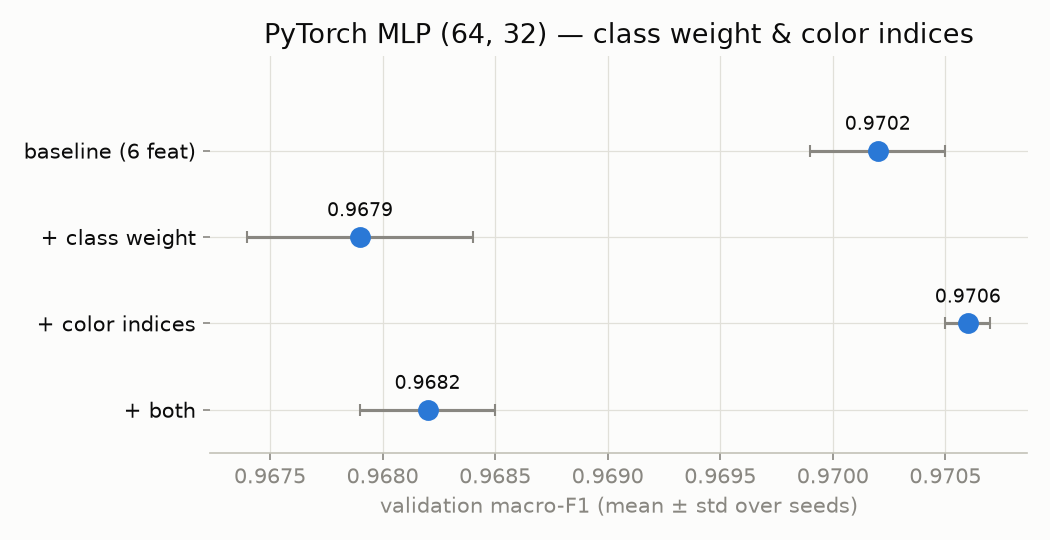
\includegraphics[width=0.8\textwidth]{torch_improvements.png}
\caption{절제 실험: 구성별 검증 macro-F1 (시드 3개 평균 $\pm$ 표준편차).}
\label{fig:ablation}
\end{figure}

PyTorch 재구현 기본 구성(0.9702)은 scikit-learn 구현(0.9681)보다 이미 높았는데,
이는 검증 macro-F1을 직접 관찰하는 조기 종료의 차이로 추정된다. 클래스 가중치는
QSO 재현율을 $+1.3$\%p 올리지만 다른 클래스의 정밀도를 낮춰 macro-F1은 오히려
하락하는 트레이드오프를 보였다. 반면 색지수는 작지만 일관된 개선을
보였고(시드 표준편차 0.0001로 안정적) QSO 재현율도 함께 개선되어, \textbf{색지수를
포함한 특성 10개 구성(클래스 가중치 없음)}을 최종 구성으로 확정하였다.

최종 구성을 보류해 둔 시험 세트 20{,}000건에서 평가한 결과 \textbf{macro-F1
$0.9700 \pm 0.0002$, 정확도 0.9737}을 얻었다. 클래스별 F1은 GALAXY 0.978,
STAR 0.985, QSO 0.947이며, 검증과 시험 성능이 거의 같아 과적합 징후는 없다.

\section{과반수 투표 앙상블}

시드에 따른 성능 변동을 제거하기 위해, 최종 구성의 모델 10개를 매 실행마다
새로 추출하는 무작위 시드로 학습하고 hard majority voting(동점은 낮은 클래스
인덱스)으로 결합하였다(그림~\ref{fig:ensemble}).

\begin{figure}[htbp]
\centering
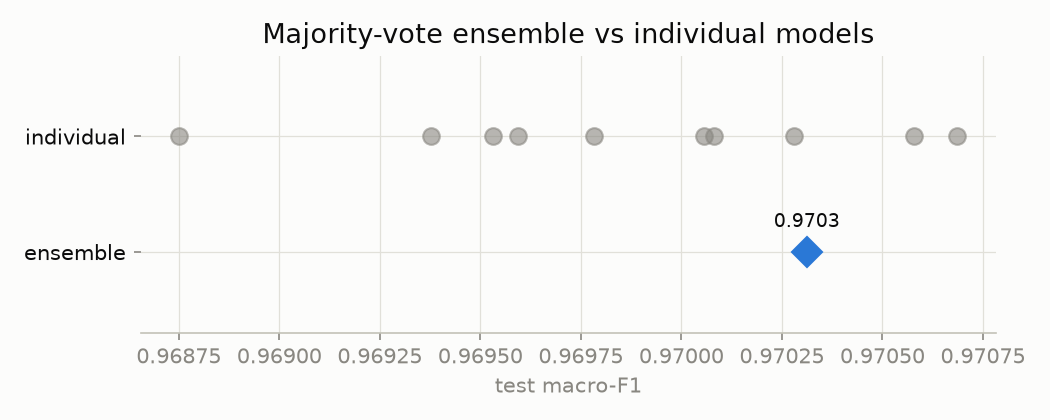
\includegraphics[width=0.8\textwidth]{ensemble_comparison.png}
\caption{개별 모델 10개와 과반수 투표 앙상블의 시험 macro-F1 비교.}
\label{fig:ensemble}
\end{figure}

개별 모델의 시험 macro-F1은 $0.9699 \pm 0.0006$(범위 $[0.9688,\,0.9707]$)이었고,
앙상블은 \textbf{macro-F1 0.9703, 정확도 0.9741}로 개별 평균을 상회하며 10개 중
8개 모델보다 높았다. 개선 폭 자체는 크지 않은데, 단일 모델이 이미 안정적이어서
투표로 정정할 오류가 많지 않기 때문이다. 앙상블의 실질적 이득은 시드 선택에 따라
0.9688까지 내려갈 수 있는 하방 위험의 제거이며, 비용은 학습·추론 10배이다. 성능
안정성이 최우선이면 앙상블을, 단순함이 우선이면 단일 모델(0.9700)을 권장한다.

\section{결론 및 향후 과제}

데이터 탐색을 통해 결측 1행 삭제, 이상치 미제거, 특성 선택,
RobustScaler/$\log(1+x)$ 스케일링의 전처리 방침을 수립하고, 깊이 비교 실험으로
은닉층 2개 (64, 32) 구조를 채택하였다. PyTorch 절제 실험에서 색지수 파생 특성을
채택해(클래스 가중치는 macro-F1 기준 기각) 시험 macro-F1 0.9700의 최종 단일
모델을 얻었고, 무작위 시드 10개 모델의 과반수 투표 앙상블로 시험 macro-F1
0.9703과 시드 간 변동 제거를 확인하였다. 향후 과제는 다음과 같다.

\begin{itemize}
  \item 최종 구성 모델의 저장·추론 코드 정리
  \item 하이퍼파라미터 미세 조정(은닉 크기, dropout, 학습률 스케줄)을 통한
        QSO F1 추가 개선 여지 탐색
  \item QSO 재현율이 우선인 시나리오에서의 클래스 가중치 재고려
        (macro-F1 $-0.2$\%p 트레이드오프)
\end{itemize}

\end{document}
